\documentclass[11pt]{article}
\usepackage[a4paper,margin=0.8in]{geometry}
\usepackage{amsmath,amssymb,bm}
\usepackage{graphicx}
\usepackage{booktabs}
\usepackage{float}
\usepackage[hypertexnames=false]{hyperref}

\title{Corrected PROM Case 2 Oracle Diagnostic}
\author{S. Ares de Parga}
\date{\today}

\begin{document}
\maketitle

\section*{Purpose}
This diagnostic isolates the online structure of PROM--ANN Case~2.  All results
are PROM-only; no HPROM or ECSW online data are used.  The corresponding
linear PROM trajectory is used as the coefficient reference for each basis.  The
Case~2 manifold has the form
\begin{equation*}
\widetilde{\mathbf u}
=
\mathbf u_{\mathrm{ref}}
+
\mathbf V\mathbf q
+
\overline{\mathbf V}\overline{\mathbf q}(t),
\end{equation*}
where the online solve determines only $\mathbf q$.  The oracle variants set
$\overline{\mathbf q}(t)=\overline{\mathbf q}^{\mathrm{lin}}(t)$ from the
linear PROM trajectory and therefore remove secondary-coordinate regression
error.  Any remaining discrepancy with the linear PROM measures the online
reduced problem itself.

\paragraph{Status of the test.}
The corrected diagnostic has been run for the four evaluation parameters
$\boldsymbol\mu^{(v)}$, $\boldsymbol\mu^{(1)}$,
$\boldsymbol\mu^{(2)}$, and $\boldsymbol\mu^{(3)}$, using both the
MLSPG-sensitive basis and the Euclidean POD basis.  The tables and figures
below summarize the completed PROM-only checks.

\paragraph{Initialization used in this corrected diagnostic.}
For Case~2, the initial primary coordinate must account for the prescribed
secondary block.  The diagnostic therefore initializes
\begin{equation*}
\mathbf q(0)
=
\arg\min_{\mathbf y}
\left\|
\mathbf V\mathbf y
-
\left(
\mathbf u_0-\mathbf u_{\mathrm{ref}}
-
\overline{\mathbf V}\,\overline{\mathbf q}(0)
\right)
\right\|_2 .
\end{equation*}
This is essential for non-Euclidean or metric-weighted bases, where
$\mathbf V^T\overline{\mathbf V}$ need not vanish in the Euclidean inner
product.

\paragraph{PG-oracle variant.}
The PG-oracle variant uses the same oracle secondary coordinates, but tests the
residual with the full linear PROM tangent before solving the overdetermined
least-squares problem for the ten primary unknowns.  This diagnostic is intended
to distinguish secondary-coordinate regression error from low/high coupling and
projection effects.


\section*{MLSPG-sensitive basis}
This section compares ANN Case~2 PROM, oracle Case~2 PROM, and PG-oracle Case~2 PROM
against the corresponding linear PROM reference for the mlspg-sensitive basis.
In the oracle cases, only the secondary coordinates are prescribed from the
linear PROM trajectory; the primary coordinates remain online unknowns.

\begin{table}[H]
\centering
\caption{PROM Case~2 oracle comparison for the mlspg-sensitive basis.}
\label{tab:mlspg-case2-state}
\resizebox{\textwidth}{!}{\begin{tabular}{llrrrrr}
\toprule
Point & Method & $\varepsilon_u$ vs HDM (\%) & $\varepsilon_u$ vs linear PROM (\%) & $\varepsilon_q^{\rm low}$ (\%) & $\varepsilon_q^{\rm high}$ (\%) & online time (s) \\
\midrule
$\mu^{(v)}$ & Linear PROM & 0.413 & 0.000 & 0.000 & 0.000 & 1467.45 \\
 & Case 2 ANN PROM & 0.551 & 0.353 & 0.741 & 1.963 & 155.03 \\
 & Case 2 oracle PROM & 0.413 & 0.000 & 0.001 & 0.000 & 67.22 \\
 & Case 2 PG-oracle PROM & 0.413 & 0.000 & 0.001 & 0.000 & 349.38 \\
\midrule
$\mu^{(1)}$ & Linear PROM & 0.460 & 0.000 & 0.000 & 0.000 & 1237.25 \\
 & Case 2 ANN PROM & 1.235 & 1.168 & 1.560 & 10.675 & 156.24 \\
 & Case 2 oracle PROM & 0.460 & 0.000 & 0.001 & 0.000 & 69.30 \\
 & Case 2 PG-oracle PROM & 0.460 & 0.000 & 0.001 & 0.000 & 342.99 \\
\midrule
$\mu^{(2)}$ & Linear PROM & 0.472 & 0.000 & 0.000 & 0.000 & 1206.89 \\
 & Case 2 ANN PROM & 1.265 & 1.172 & 0.681 & 12.848 & 157.24 \\
 & Case 2 oracle PROM & 0.472 & 0.001 & 0.001 & 0.000 & 67.85 \\
 & Case 2 PG-oracle PROM & 0.472 & 0.000 & 0.001 & 0.000 & 343.28 \\
\midrule
$\mu^{(3)}$ & Linear PROM & 0.868 & 0.000 & 0.000 & 0.000 & 1244.33 \\
 & Case 2 ANN PROM & 3.868 & 3.763 & 3.760 & 44.282 & 44.05 \\
 & Case 2 oracle PROM & 0.868 & 0.000 & 0.000 & 0.000 & 68.28 \\
 & Case 2 PG-oracle PROM & 0.868 & 0.000 & 0.000 & 0.000 & 275.66 \\
\bottomrule
\end{tabular}
}
\end{table}

\begin{table}[H]
\centering
\caption{Mean PROM Case~2 oracle metrics over the four evaluation points for the mlspg-sensitive basis.}
\label{tab:mlspg-case2-mean}
\resizebox{\textwidth}{!}{\begin{tabular}{lrrrrr}
\toprule
Method & mean $\varepsilon_u$ vs HDM (\%) & mean $\varepsilon_u$ vs linear PROM (\%) & mean $\varepsilon_q^{\rm low}$ (\%) & mean $\varepsilon_q^{\rm high}$ (\%) & mean time (s) \\
\midrule
Case 2 ANN PROM & 1.730 & 1.614 & 1.685 & 17.442 & 128.14 \\
Case 2 oracle PROM & 0.553 & 0.000 & 0.001 & 0.000 & 68.16 \\
Case 2 PG-oracle PROM & 0.553 & 0.000 & 0.001 & 0.000 & 327.83 \\
\bottomrule
\end{tabular}
}
\end{table}

\begin{figure}[H]
\centering
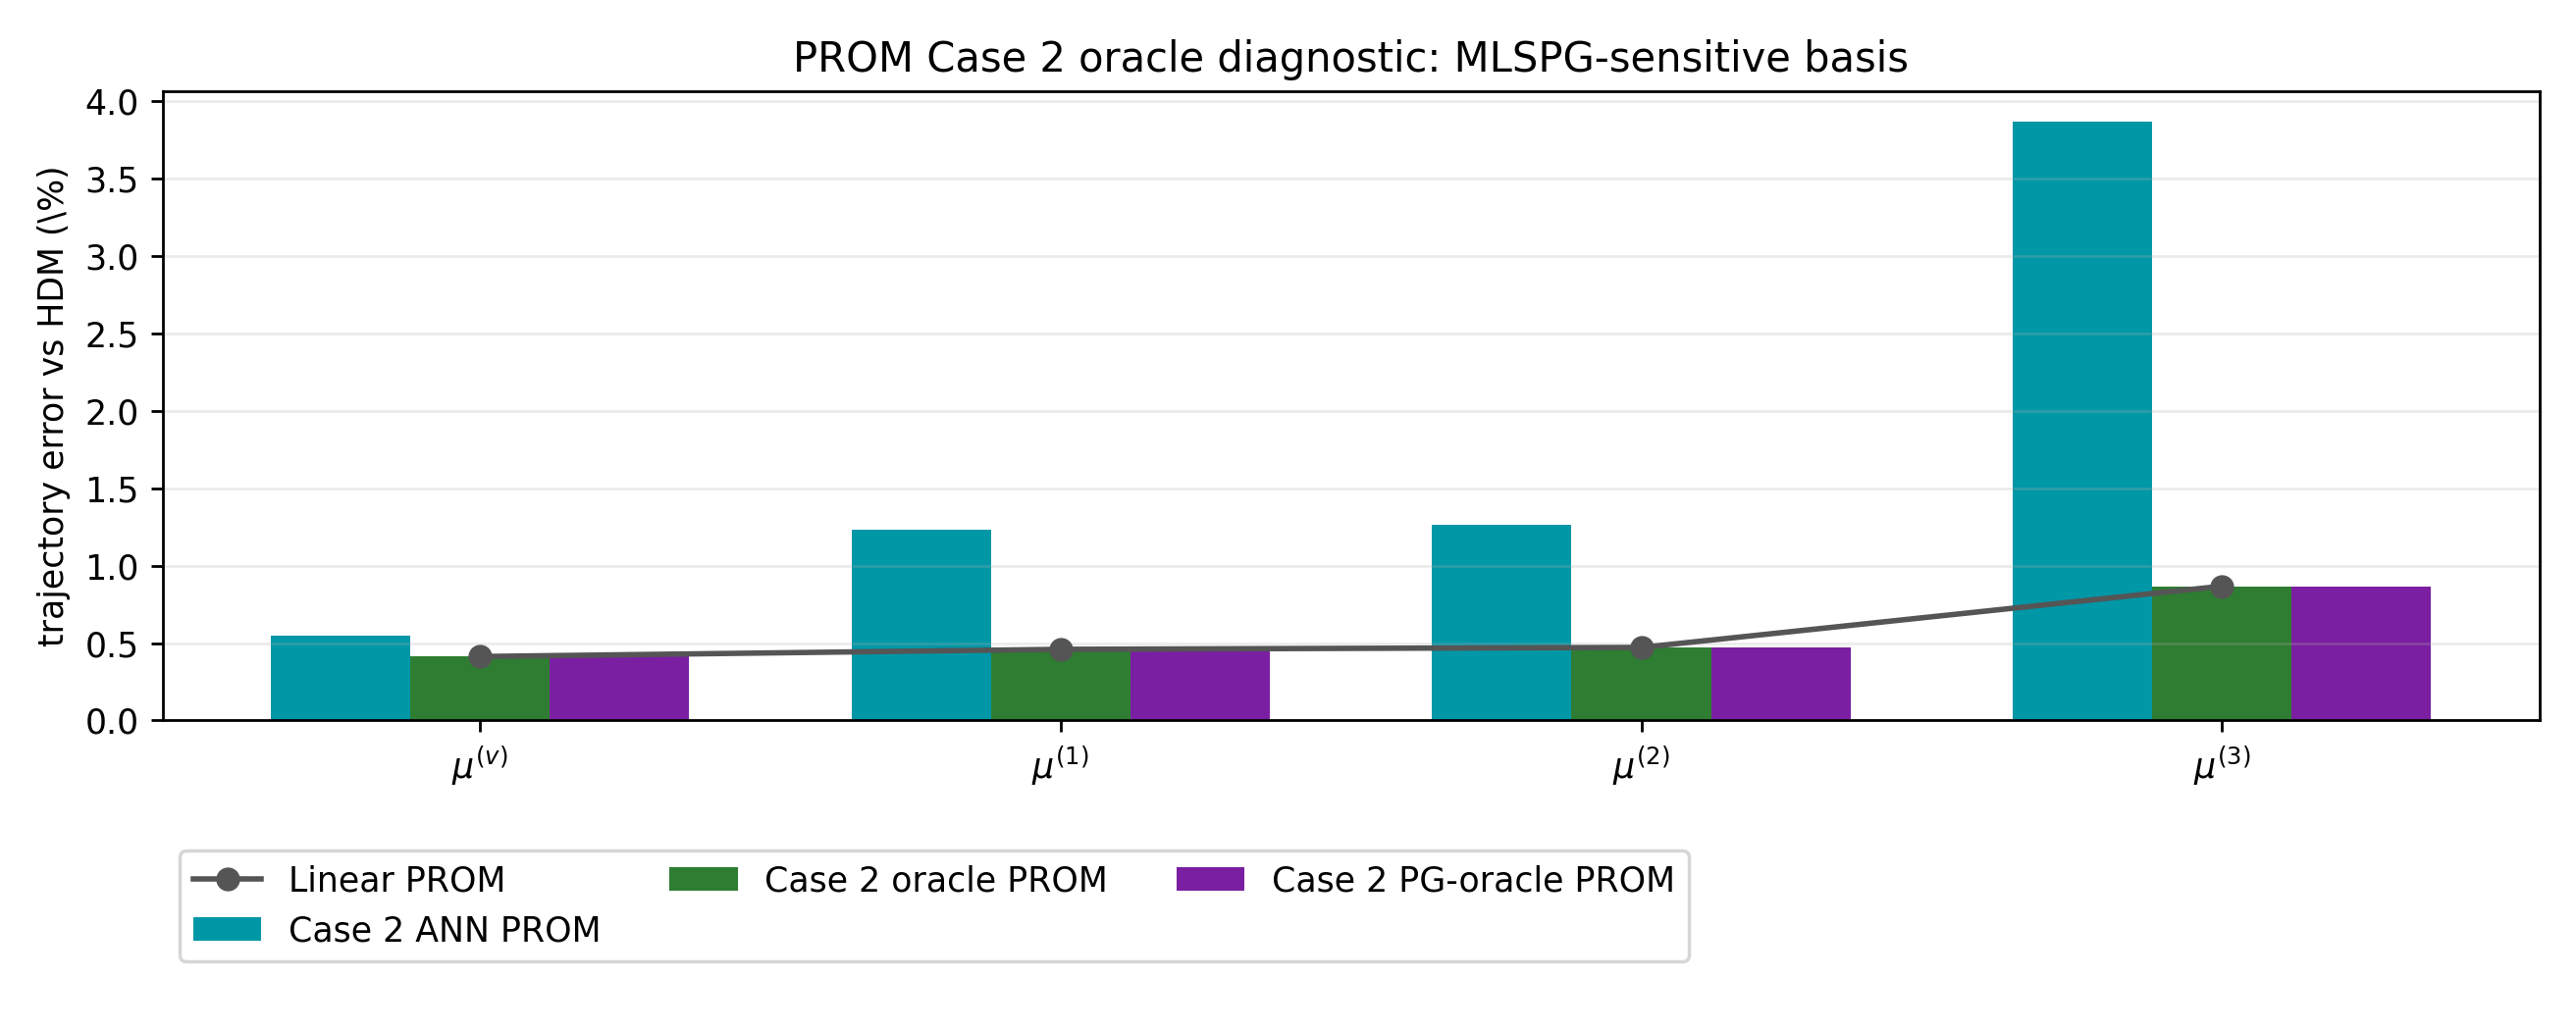
\includegraphics[width=0.92\textwidth]{figures/mlspg_case2_state_error_bars.png}
\caption{State-space trajectory error versus HDM for the mlspg-sensitive basis.}
\end{figure}

\begin{figure}[H]
\centering
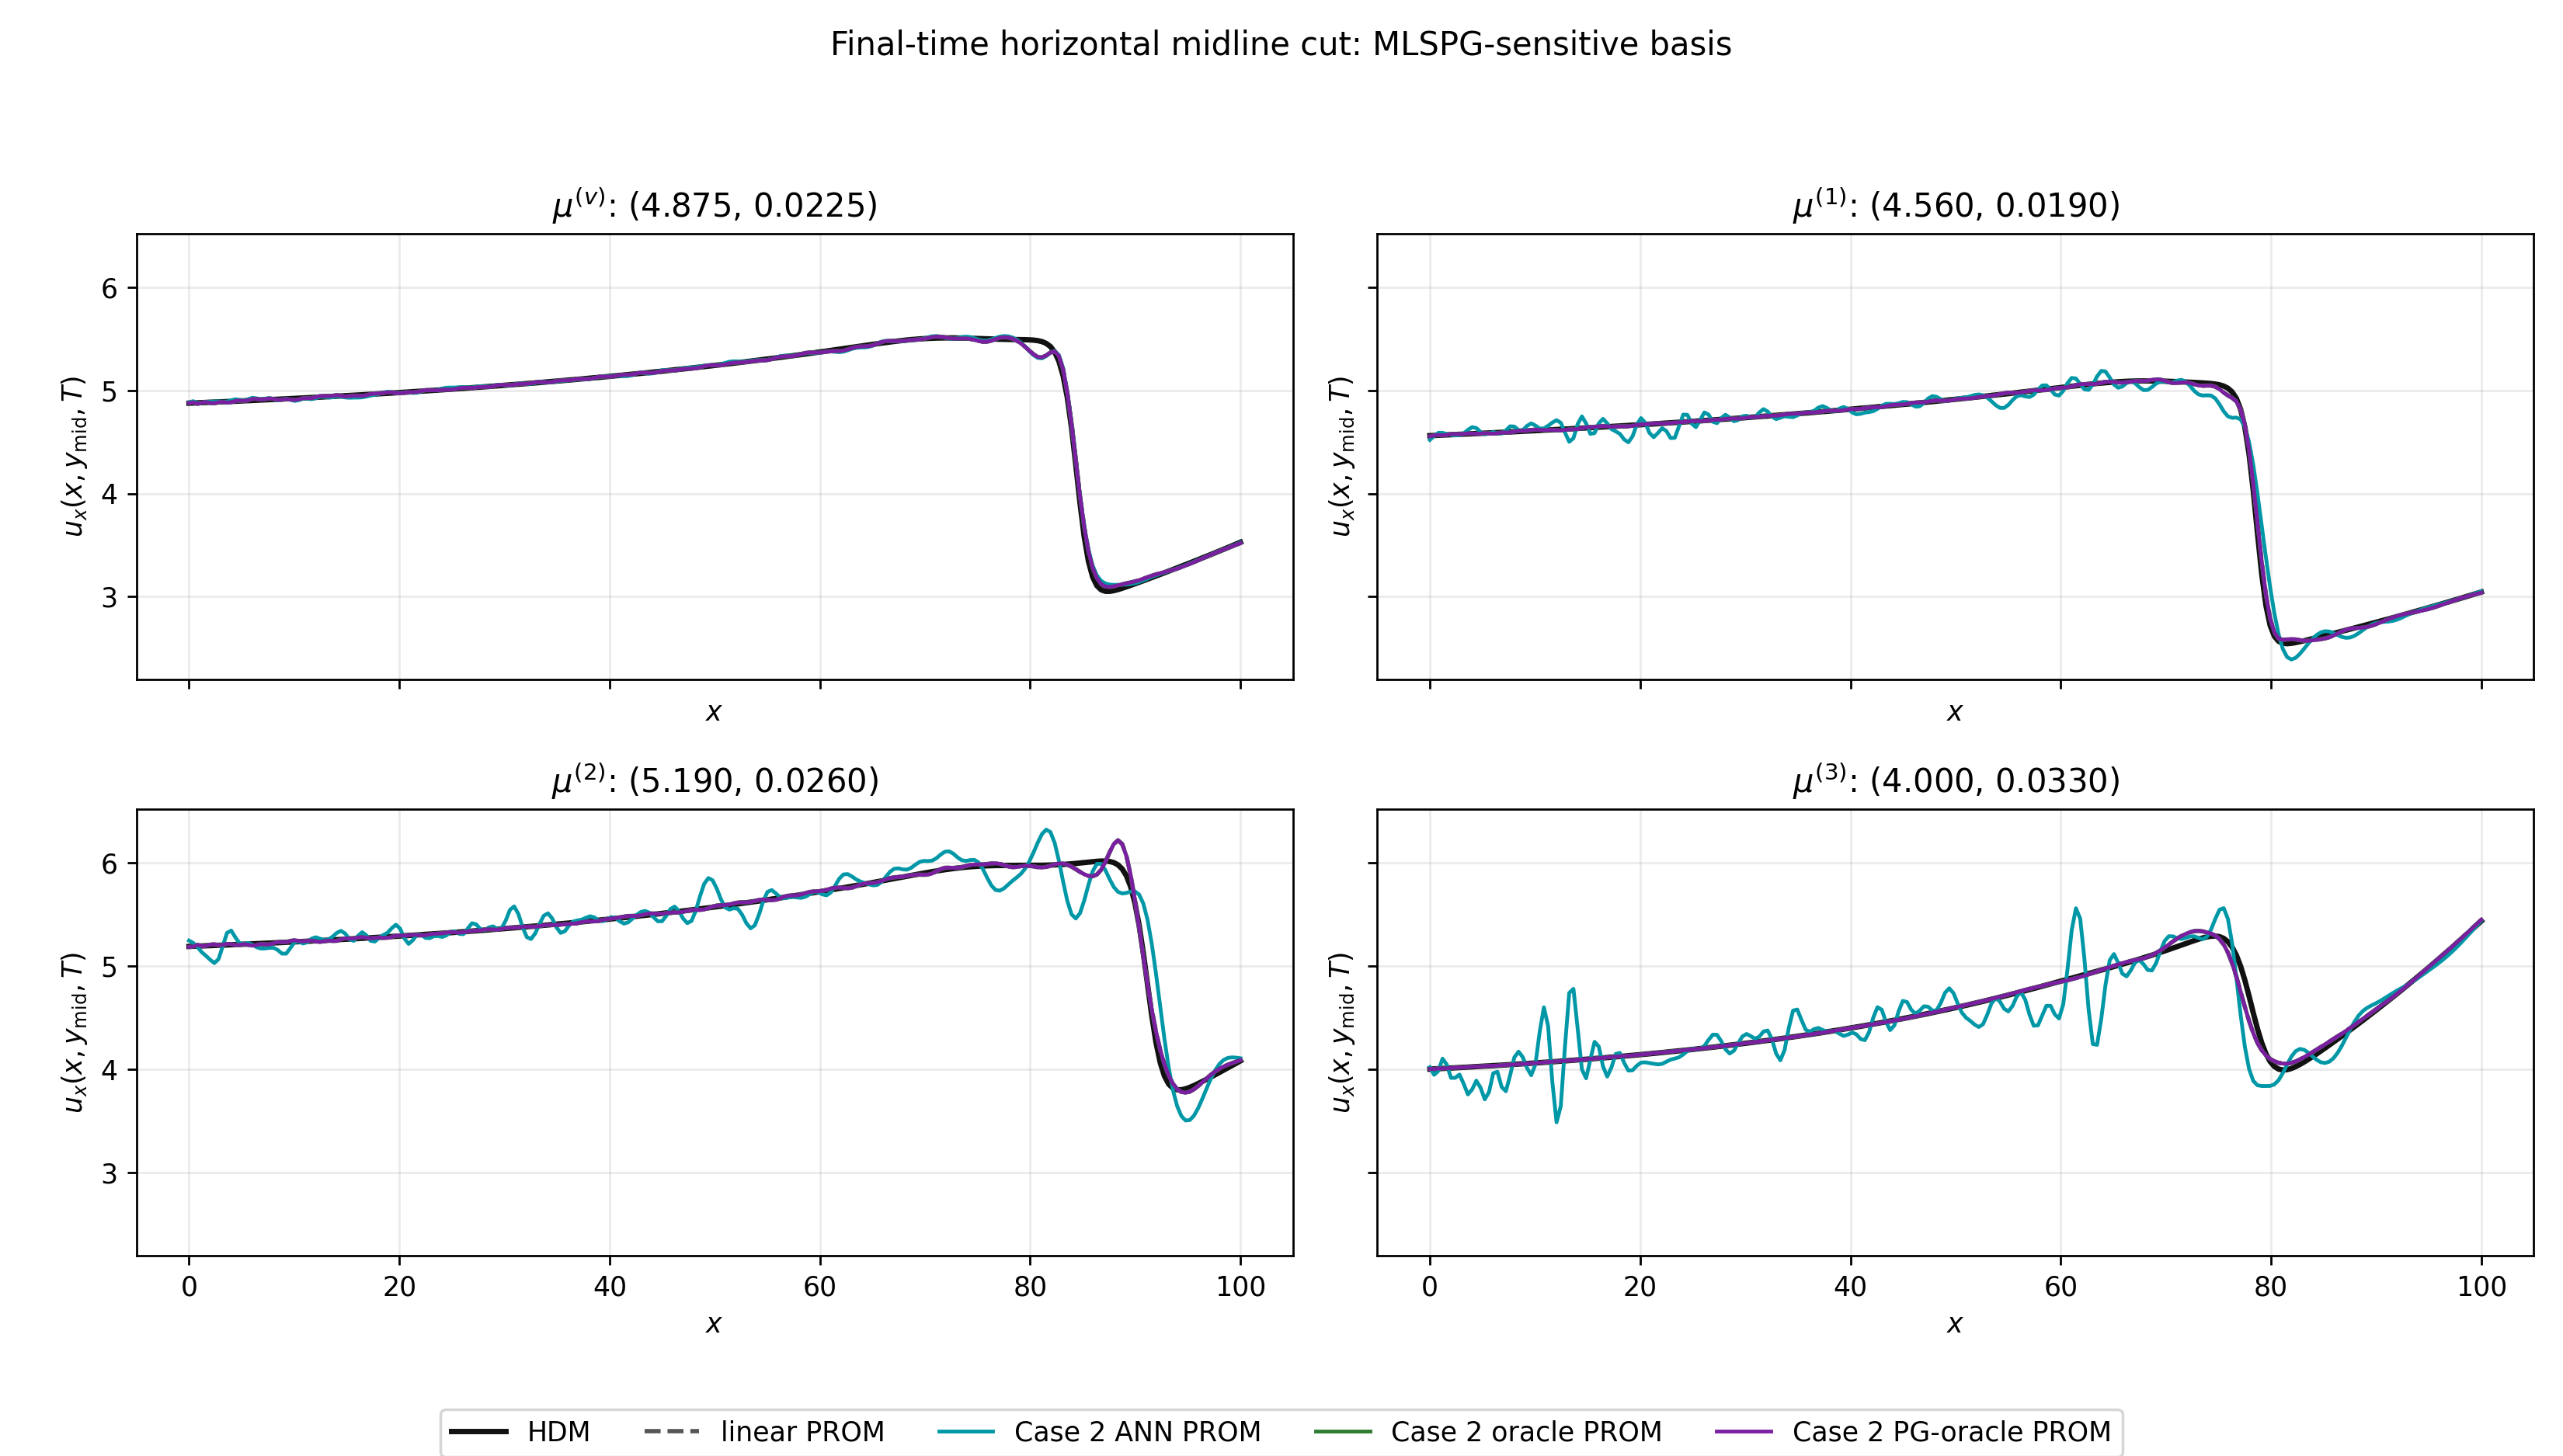
\includegraphics[width=0.98\textwidth]{figures/mlspg_case2_final_midline_overlays.png}
\caption{Final-time horizontal midline cuts of $u_x$ for HDM, linear PROM, and the Case~2 diagnostic variants for the mlspg-sensitive basis.}
\end{figure}

\begin{figure}[H]
\centering
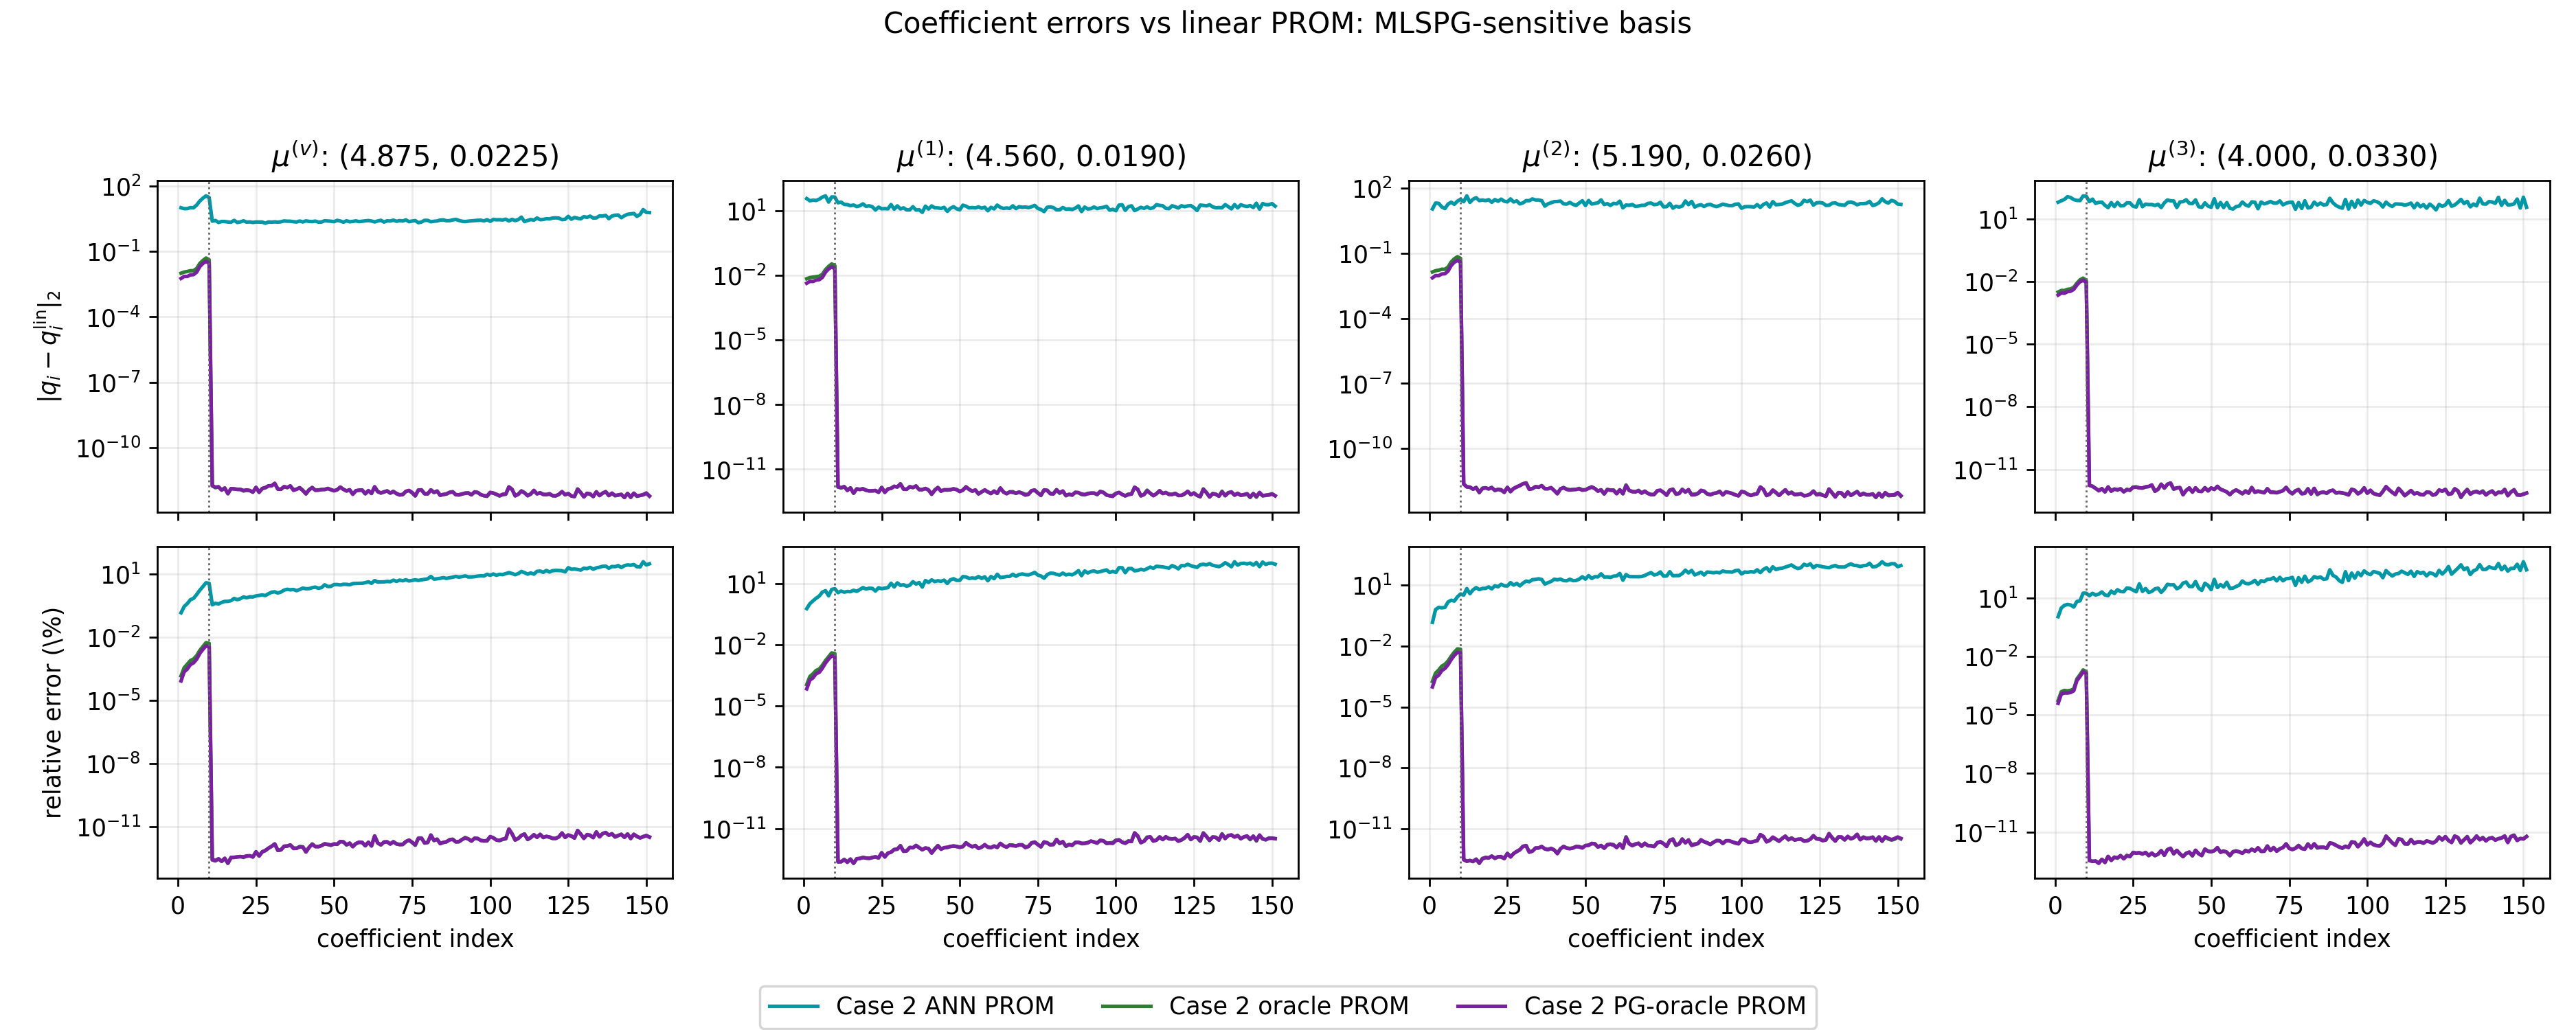
\includegraphics[width=0.98\textwidth]{figures/mlspg_case2_coeff_abs_rel_curves.png}
\caption{Per-coefficient absolute and relative errors with respect to the linear PROM coefficient trajectory.  The dotted line marks the primary/secondary split at $n=10$.}
\end{figure}

\begin{figure}[H]
\centering
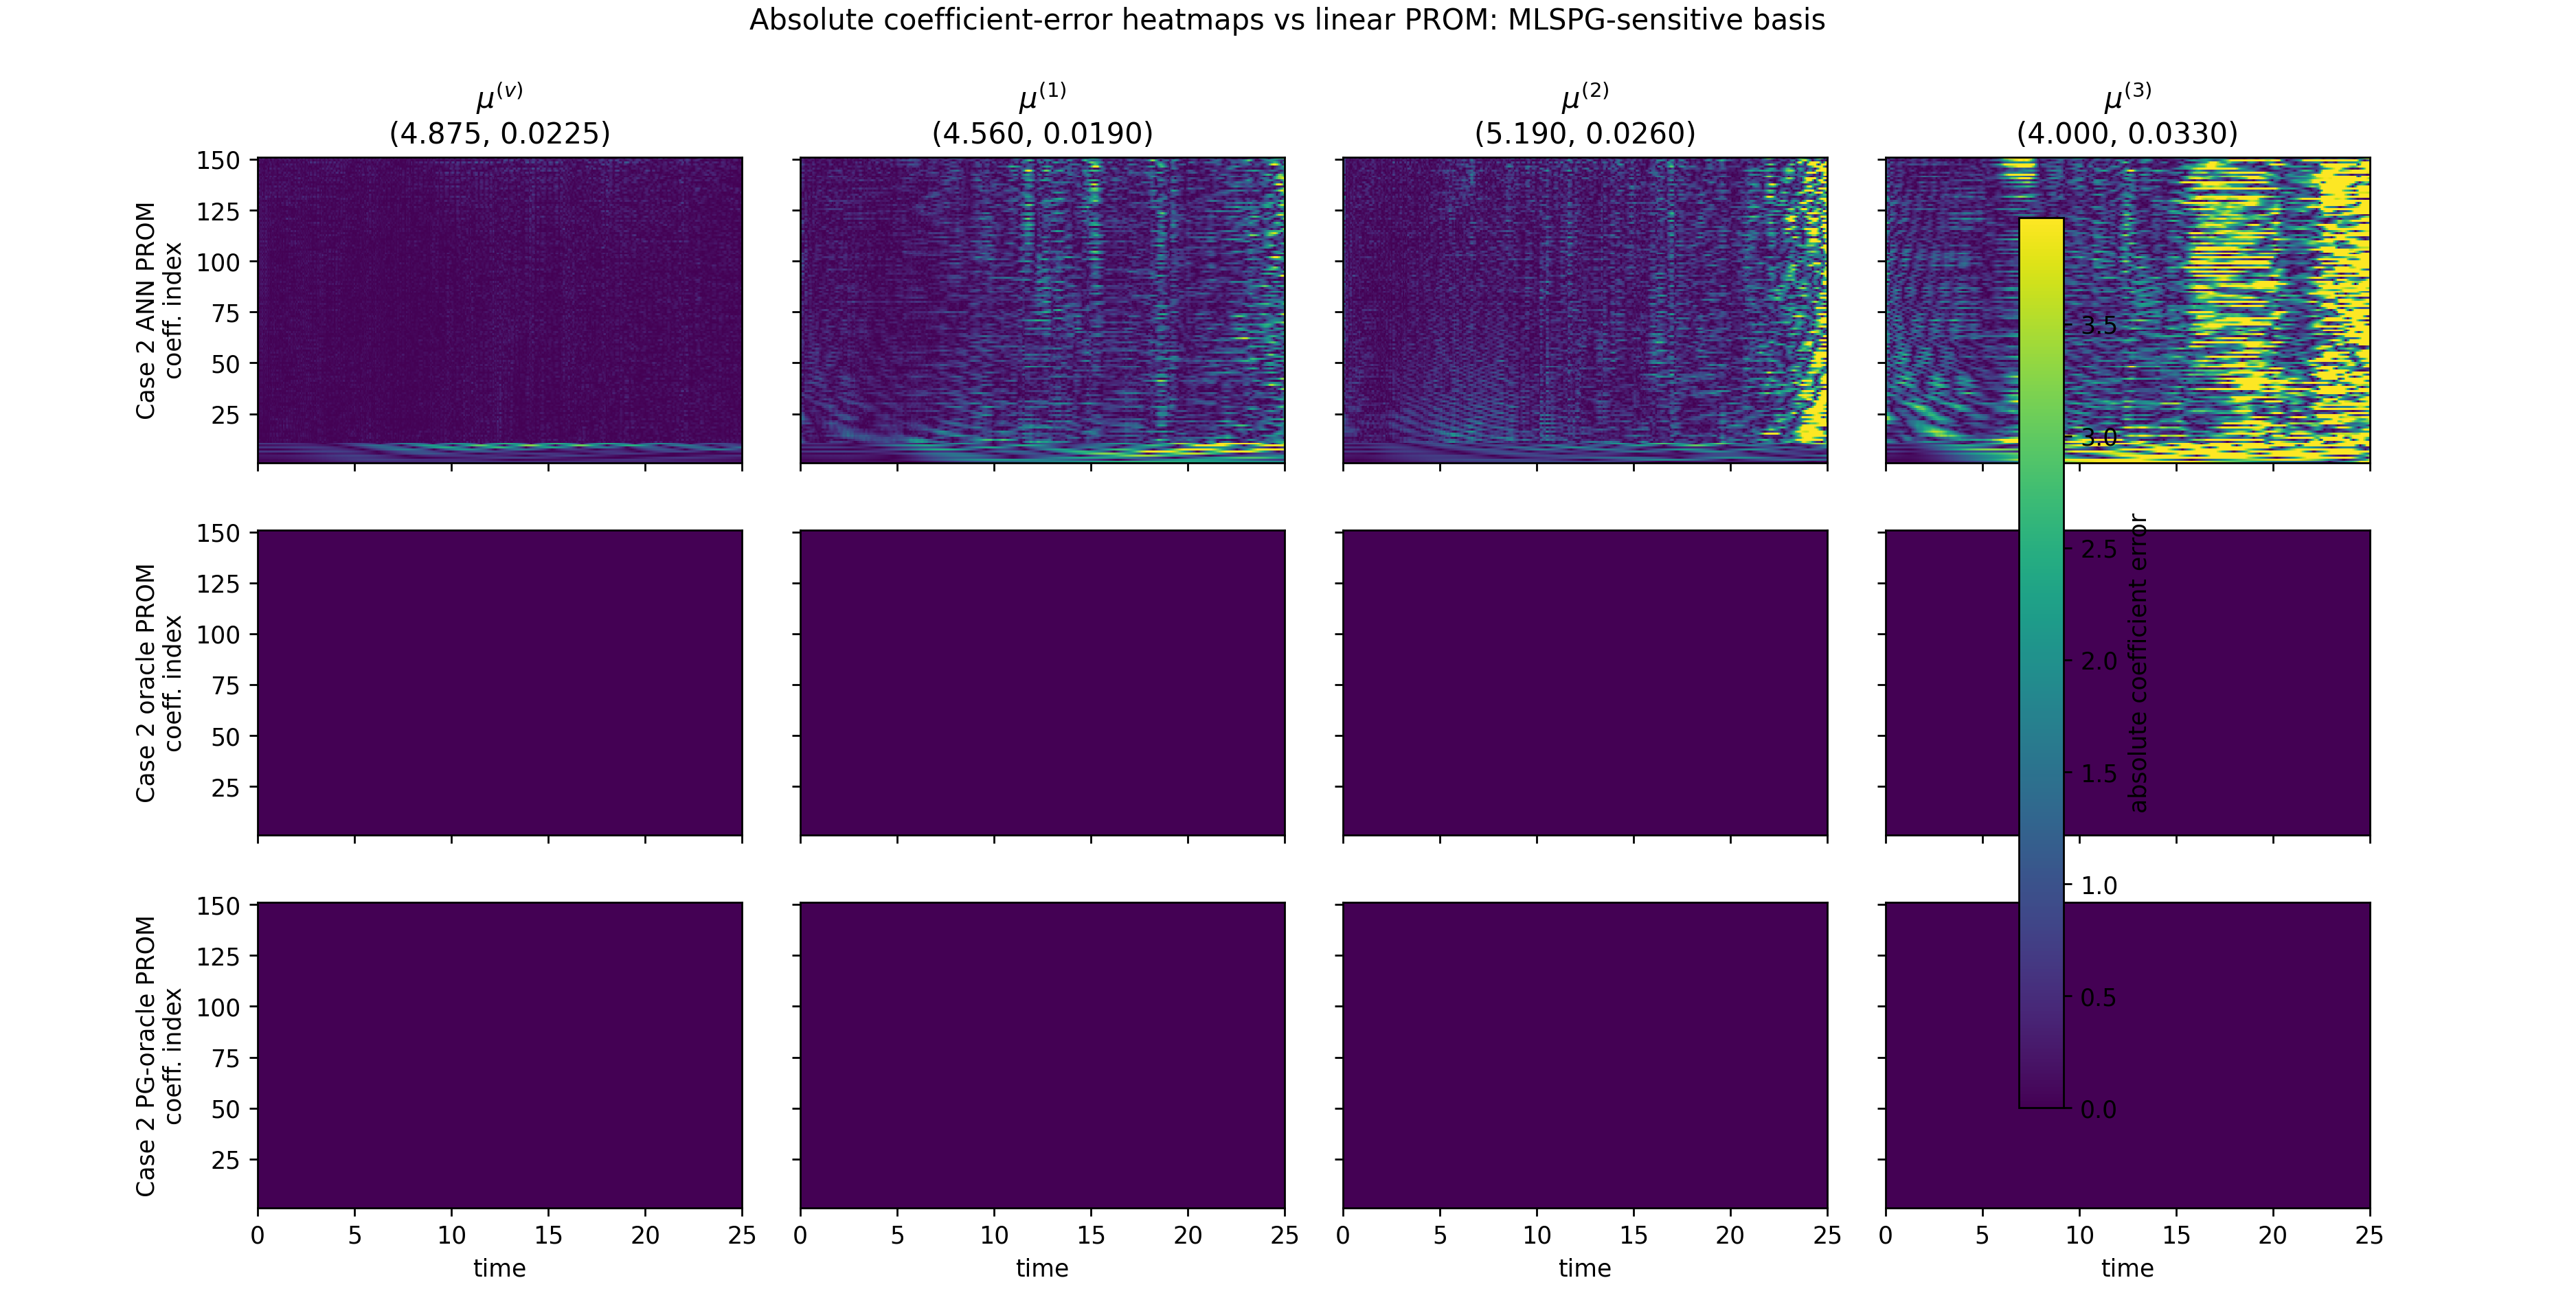
\includegraphics[width=0.98\textwidth]{figures/mlspg_case2_coeff_abs_heatmaps.png}
\caption{Absolute coefficient-error heatmaps versus the linear PROM coefficient trajectory.}
\end{figure}

\begin{figure}[H]
\centering
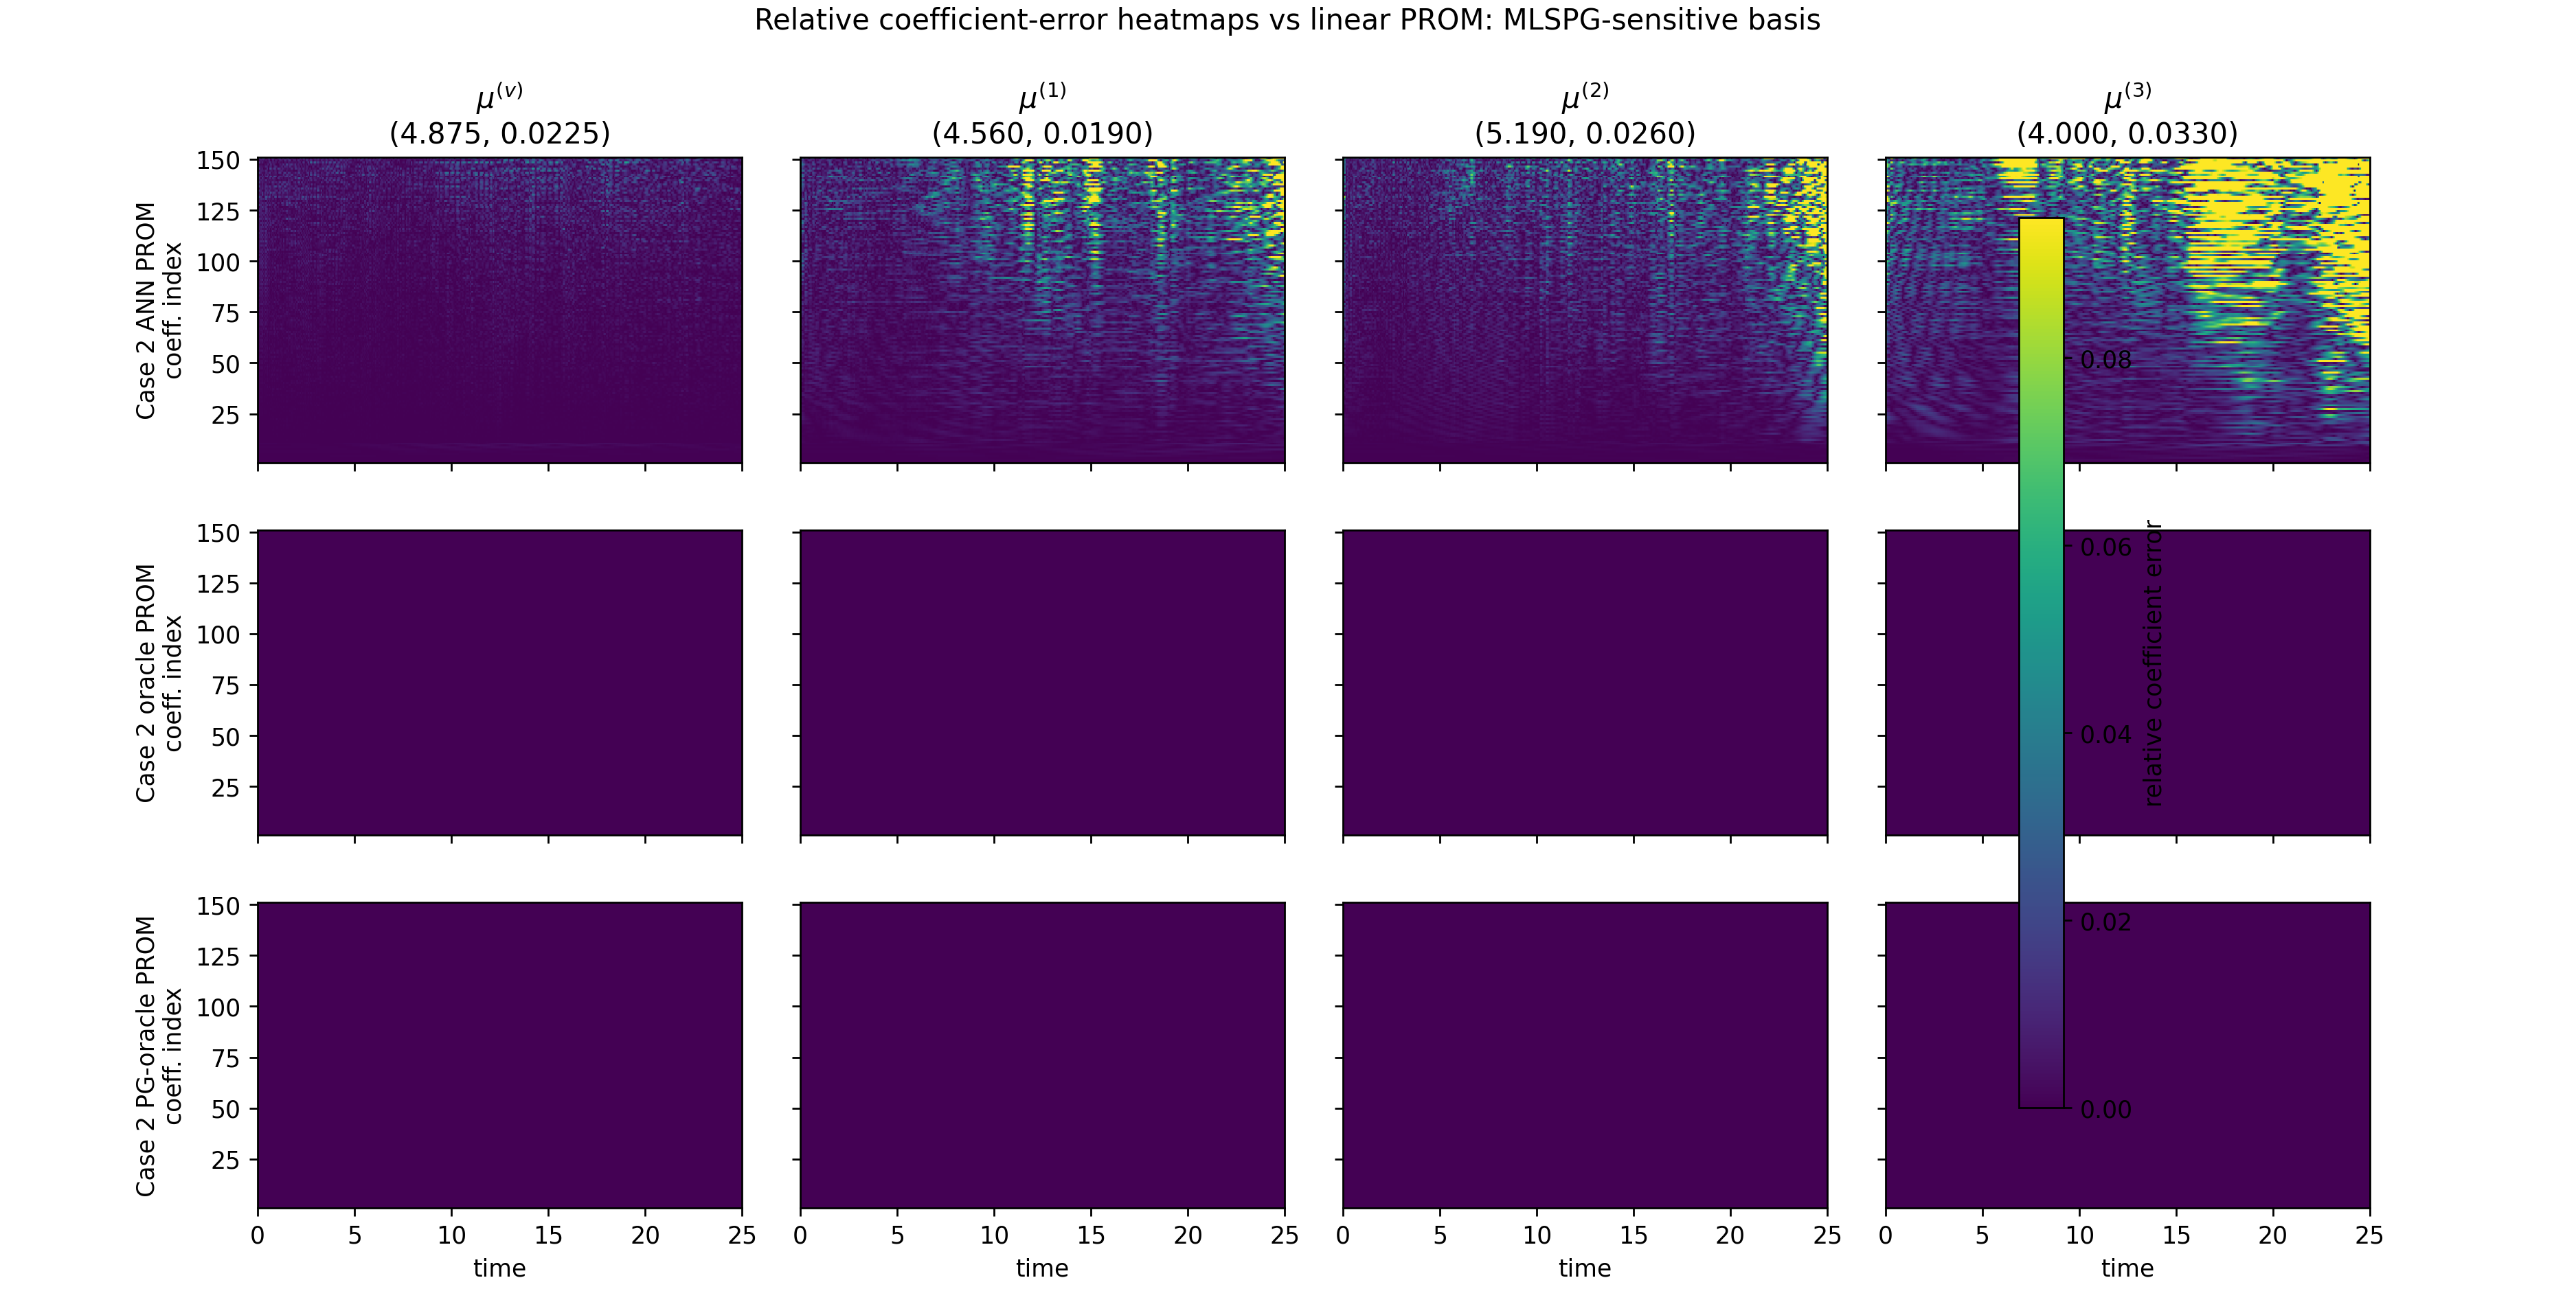
\includegraphics[width=0.98\textwidth]{figures/mlspg_case2_coeff_rel_heatmaps.png}
\caption{Relative coefficient-error heatmaps versus the linear PROM coefficient trajectory.}
\end{figure}

\paragraph{Interpretation.}
For the MLSPG-sensitive basis, the completed corrected test shows that the offset-aware initialization makes both oracle variants recover the corresponding linear PROM to approximately $10^{-4}$ percent in trajectory norm.  The earlier measurable oracle discrepancy was therefore an initialization inconsistency, not evidence that the MLSPG metric makes Case~2 structurally unable to reproduce the linear PROM when the secondary coordinates are exact.  The remaining ANN Case~2 error is therefore attributable to regression and online coupling errors, not to the oracle reduced problem.

\section*{Euclidean POD basis}
This section compares oracle Case~2 PROM, and PG-oracle Case~2 PROM
against the corresponding linear PROM reference for the euclidean pod basis.
In the oracle cases, only the secondary coordinates are prescribed from the
linear PROM trajectory; the primary coordinates remain online unknowns.

\begin{table}[H]
\centering
\caption{PROM Case~2 oracle comparison for the euclidean pod basis.}
\label{tab:euclidean-case2-state}
\resizebox{\textwidth}{!}{\begin{tabular}{llrrrrr}
\toprule
Point & Method & $\varepsilon_u$ vs HDM (\%) & $\varepsilon_u$ vs linear PROM (\%) & $\varepsilon_q^{\rm low}$ (\%) & $\varepsilon_q^{\rm high}$ (\%) & online time (s) \\
\midrule
$\mu^{(v)}$ & Linear PROM & 0.410 & 0.000 & 0.000 & 0.000 & 1370.24 \\
 & Case 2 oracle PROM & 0.410 & 0.000 & 0.001 & 0.000 & 69.32 \\
 & Case 2 PG-oracle PROM & 0.410 & 0.000 & 0.001 & 0.000 & 329.30 \\
\midrule
$\mu^{(1)}$ & Linear PROM & 0.450 & 0.000 & 0.000 & 0.000 & 1340.83 \\
 & Case 2 oracle PROM & 0.450 & 0.000 & 0.001 & 0.000 & 61.50 \\
 & Case 2 PG-oracle PROM & 0.450 & 0.000 & 0.000 & 0.000 & 321.68 \\
\midrule
$\mu^{(2)}$ & Linear PROM & 0.463 & 0.000 & 0.000 & 0.000 & 1349.99 \\
 & Case 2 oracle PROM & 0.463 & 0.000 & 0.001 & 0.000 & 61.75 \\
 & Case 2 PG-oracle PROM & 0.463 & 0.000 & 0.001 & 0.000 & 338.21 \\
\midrule
$\mu^{(3)}$ & Linear PROM & 0.850 & 0.000 & 0.000 & 0.000 & 1236.62 \\
 & Case 2 oracle PROM & 0.850 & 0.000 & 0.000 & 0.000 & 68.83 \\
 & Case 2 PG-oracle PROM & 0.850 & 0.000 & 0.000 & 0.000 & 274.48 \\
\bottomrule
\end{tabular}
}
\end{table}

\begin{table}[H]
\centering
\caption{Mean PROM Case~2 oracle metrics over the four evaluation points for the euclidean pod basis.}
\label{tab:euclidean-case2-mean}
\resizebox{\textwidth}{!}{\begin{tabular}{lrrrrr}
\toprule
Method & mean $\varepsilon_u$ vs HDM (\%) & mean $\varepsilon_u$ vs linear PROM (\%) & mean $\varepsilon_q^{\rm low}$ (\%) & mean $\varepsilon_q^{\rm high}$ (\%) & mean time (s) \\
\midrule
Case 2 oracle PROM & 0.543 & 0.000 & 0.001 & 0.000 & 65.35 \\
Case 2 PG-oracle PROM & 0.543 & 0.000 & 0.000 & 0.000 & 315.92 \\
\bottomrule
\end{tabular}
}
\end{table}

\begin{figure}[H]
\centering
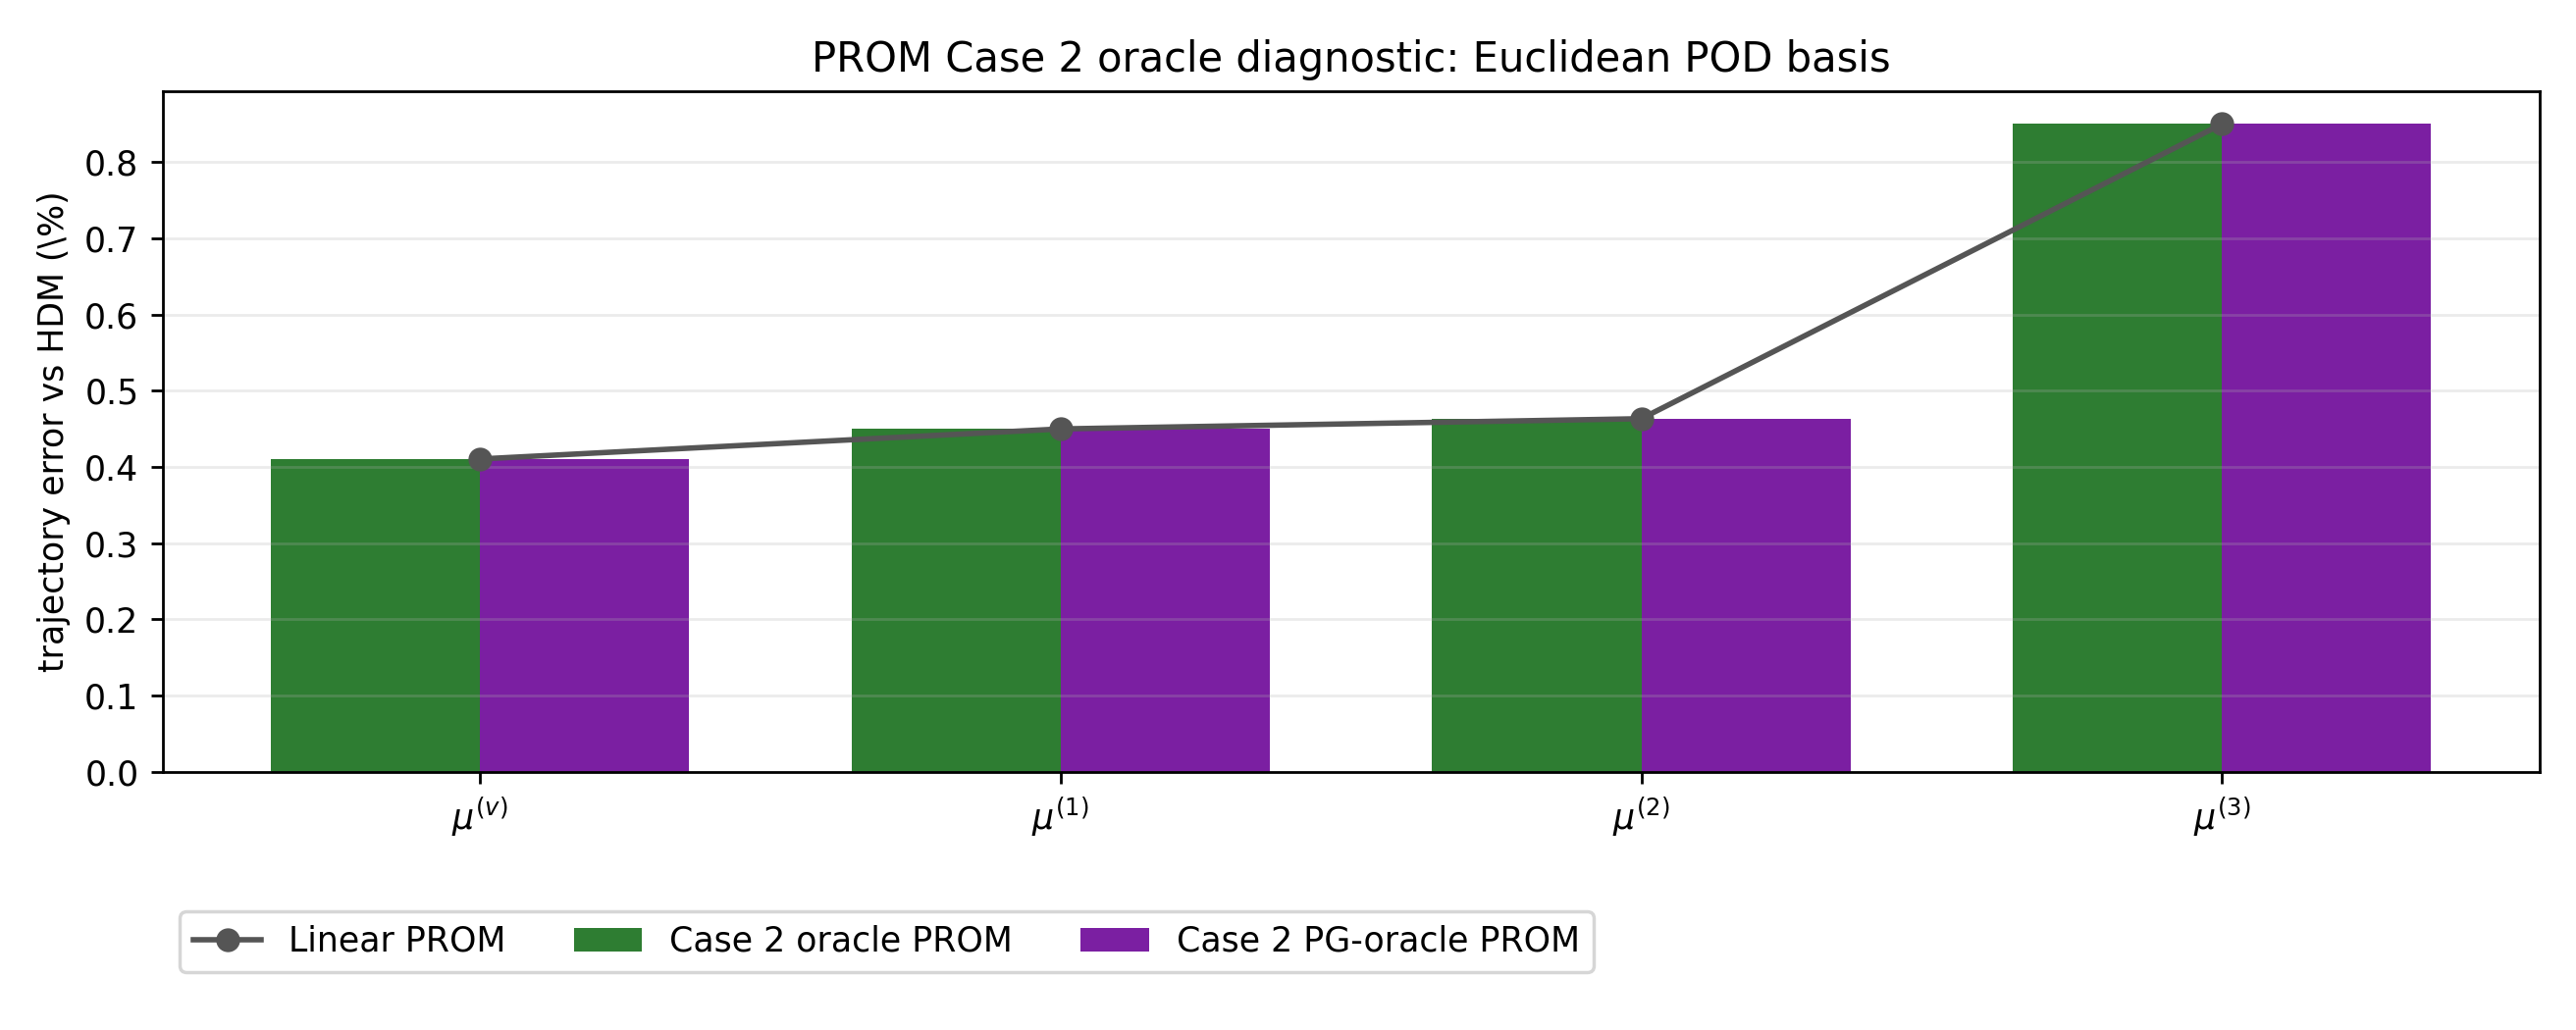
\includegraphics[width=0.92\textwidth]{figures/euclidean_case2_state_error_bars.png}
\caption{State-space trajectory error versus HDM for the euclidean pod basis.}
\end{figure}

\begin{figure}[H]
\centering
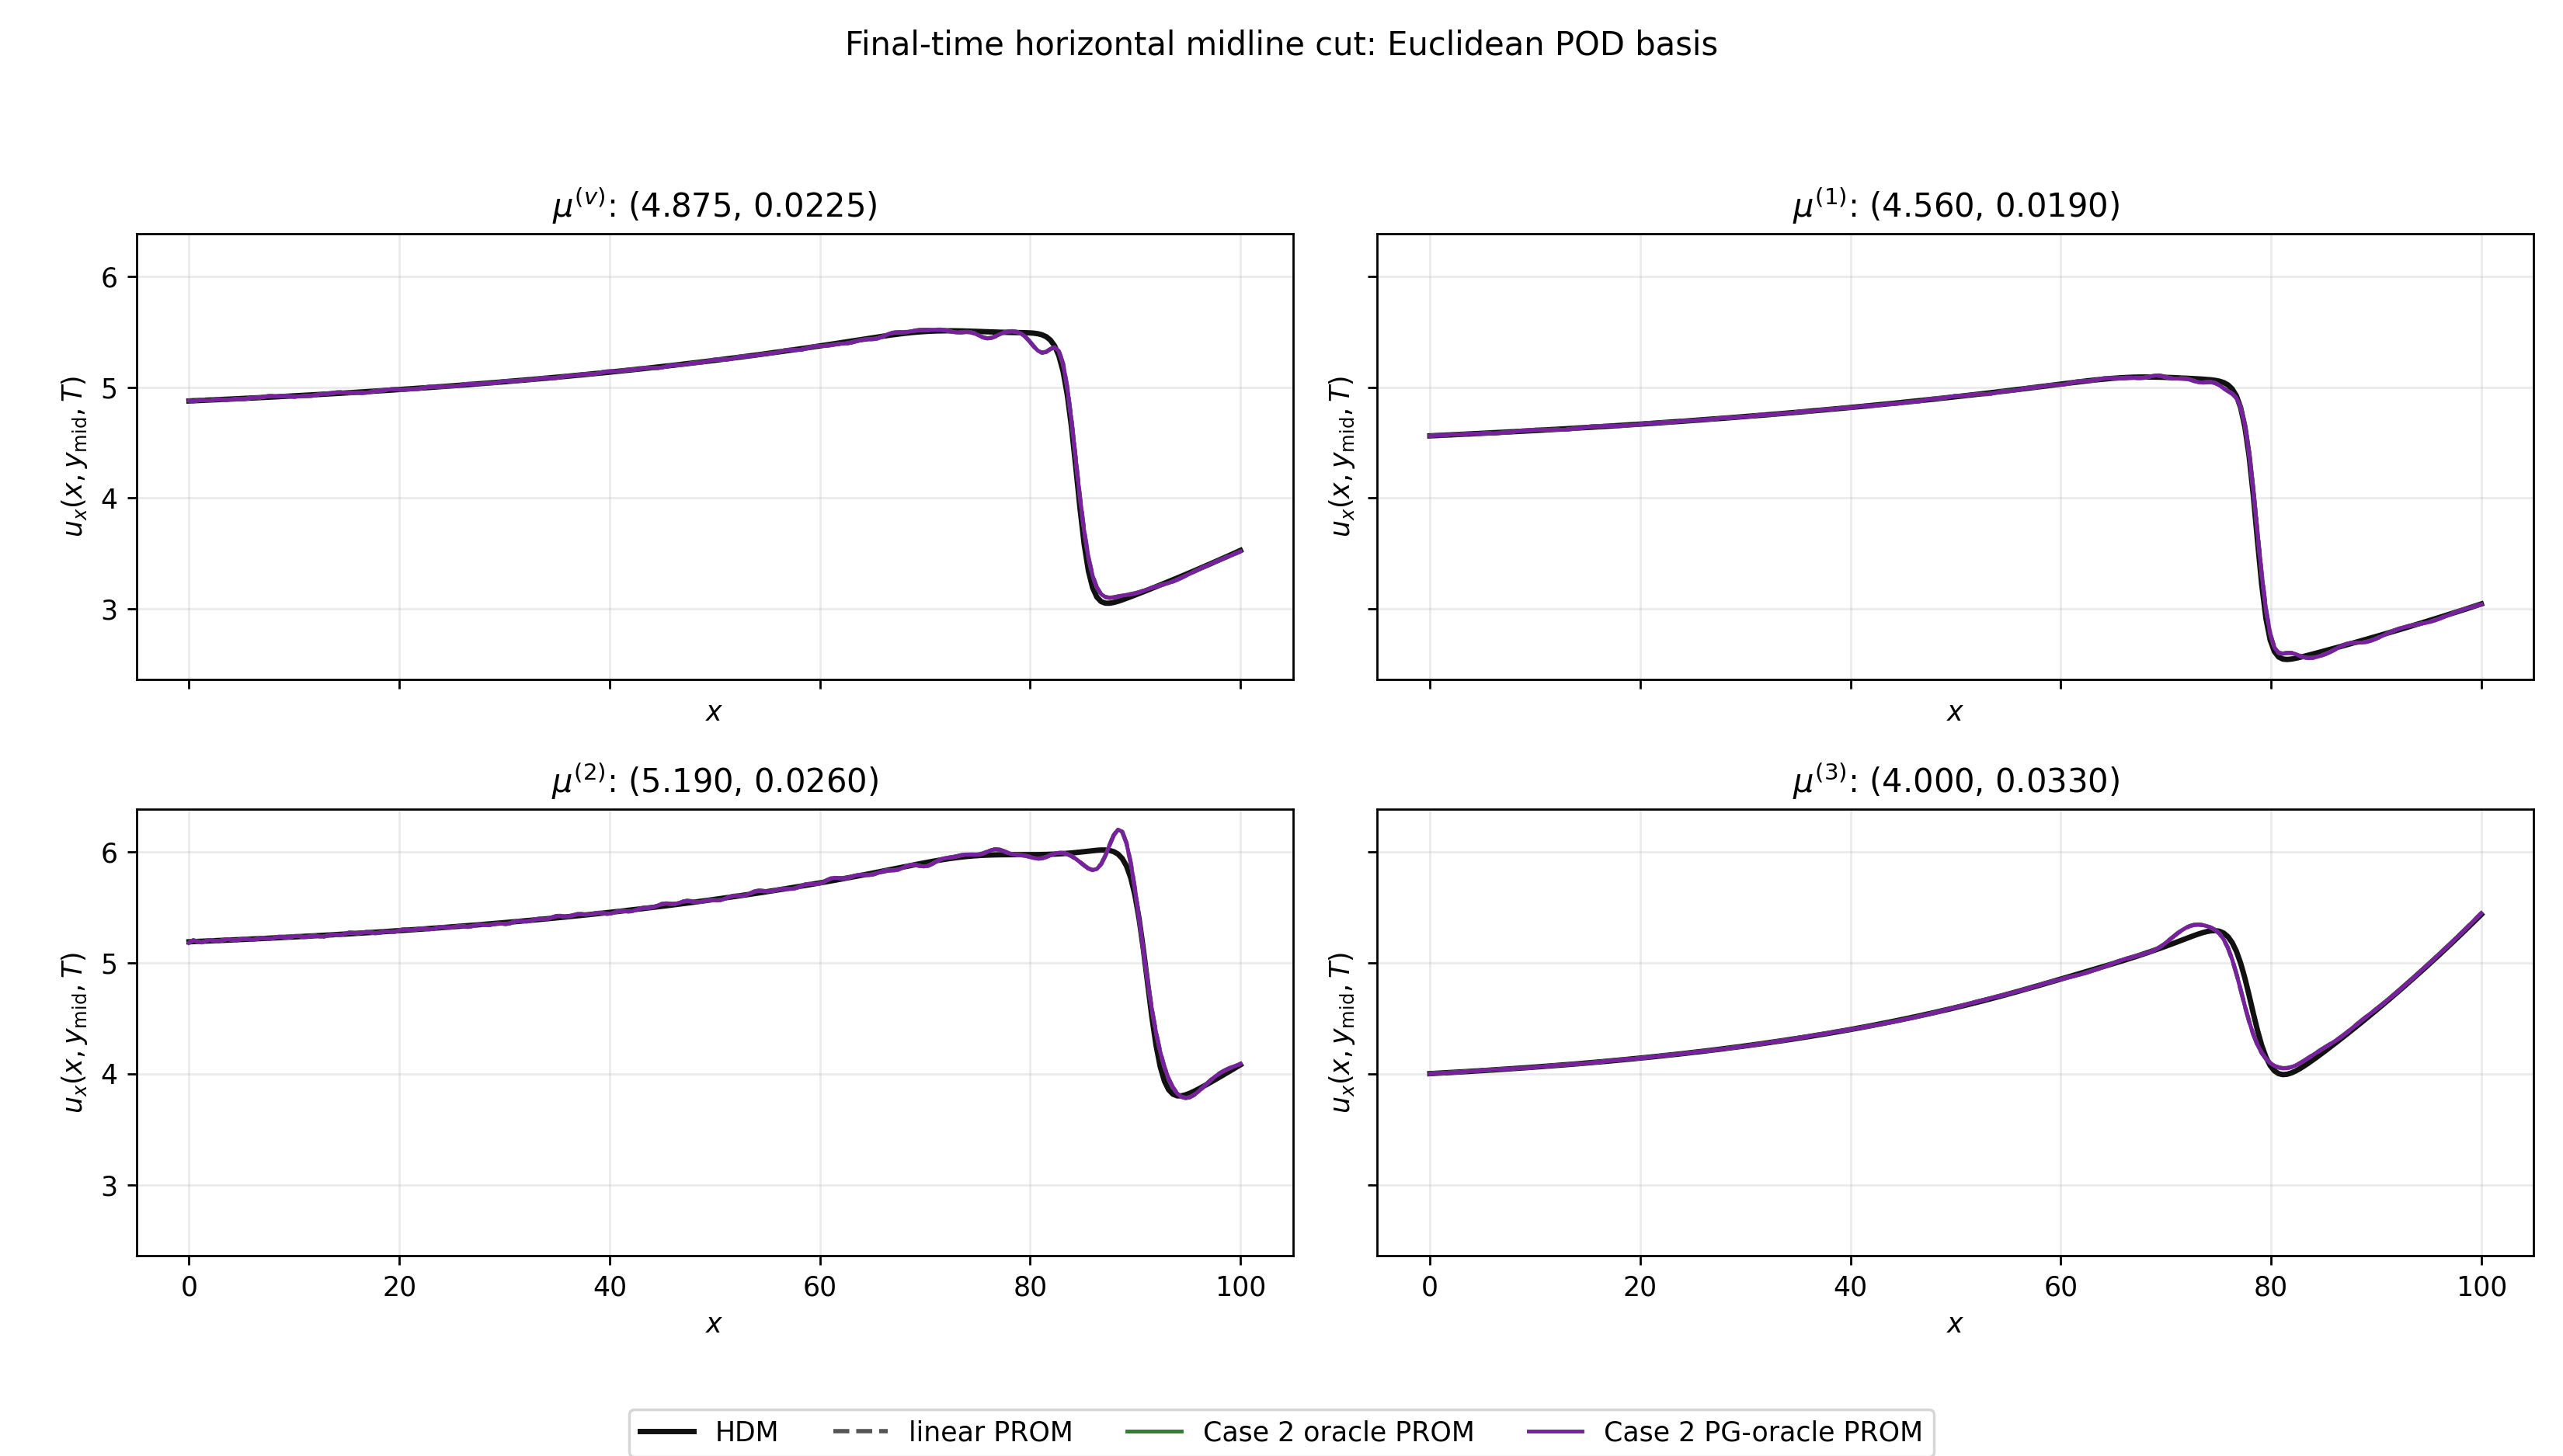
\includegraphics[width=0.98\textwidth]{figures/euclidean_case2_final_midline_overlays.png}
\caption{Final-time horizontal midline cuts of $u_x$ for HDM, linear PROM, and the Case~2 diagnostic variants for the euclidean pod basis.}
\end{figure}

\begin{figure}[H]
\centering
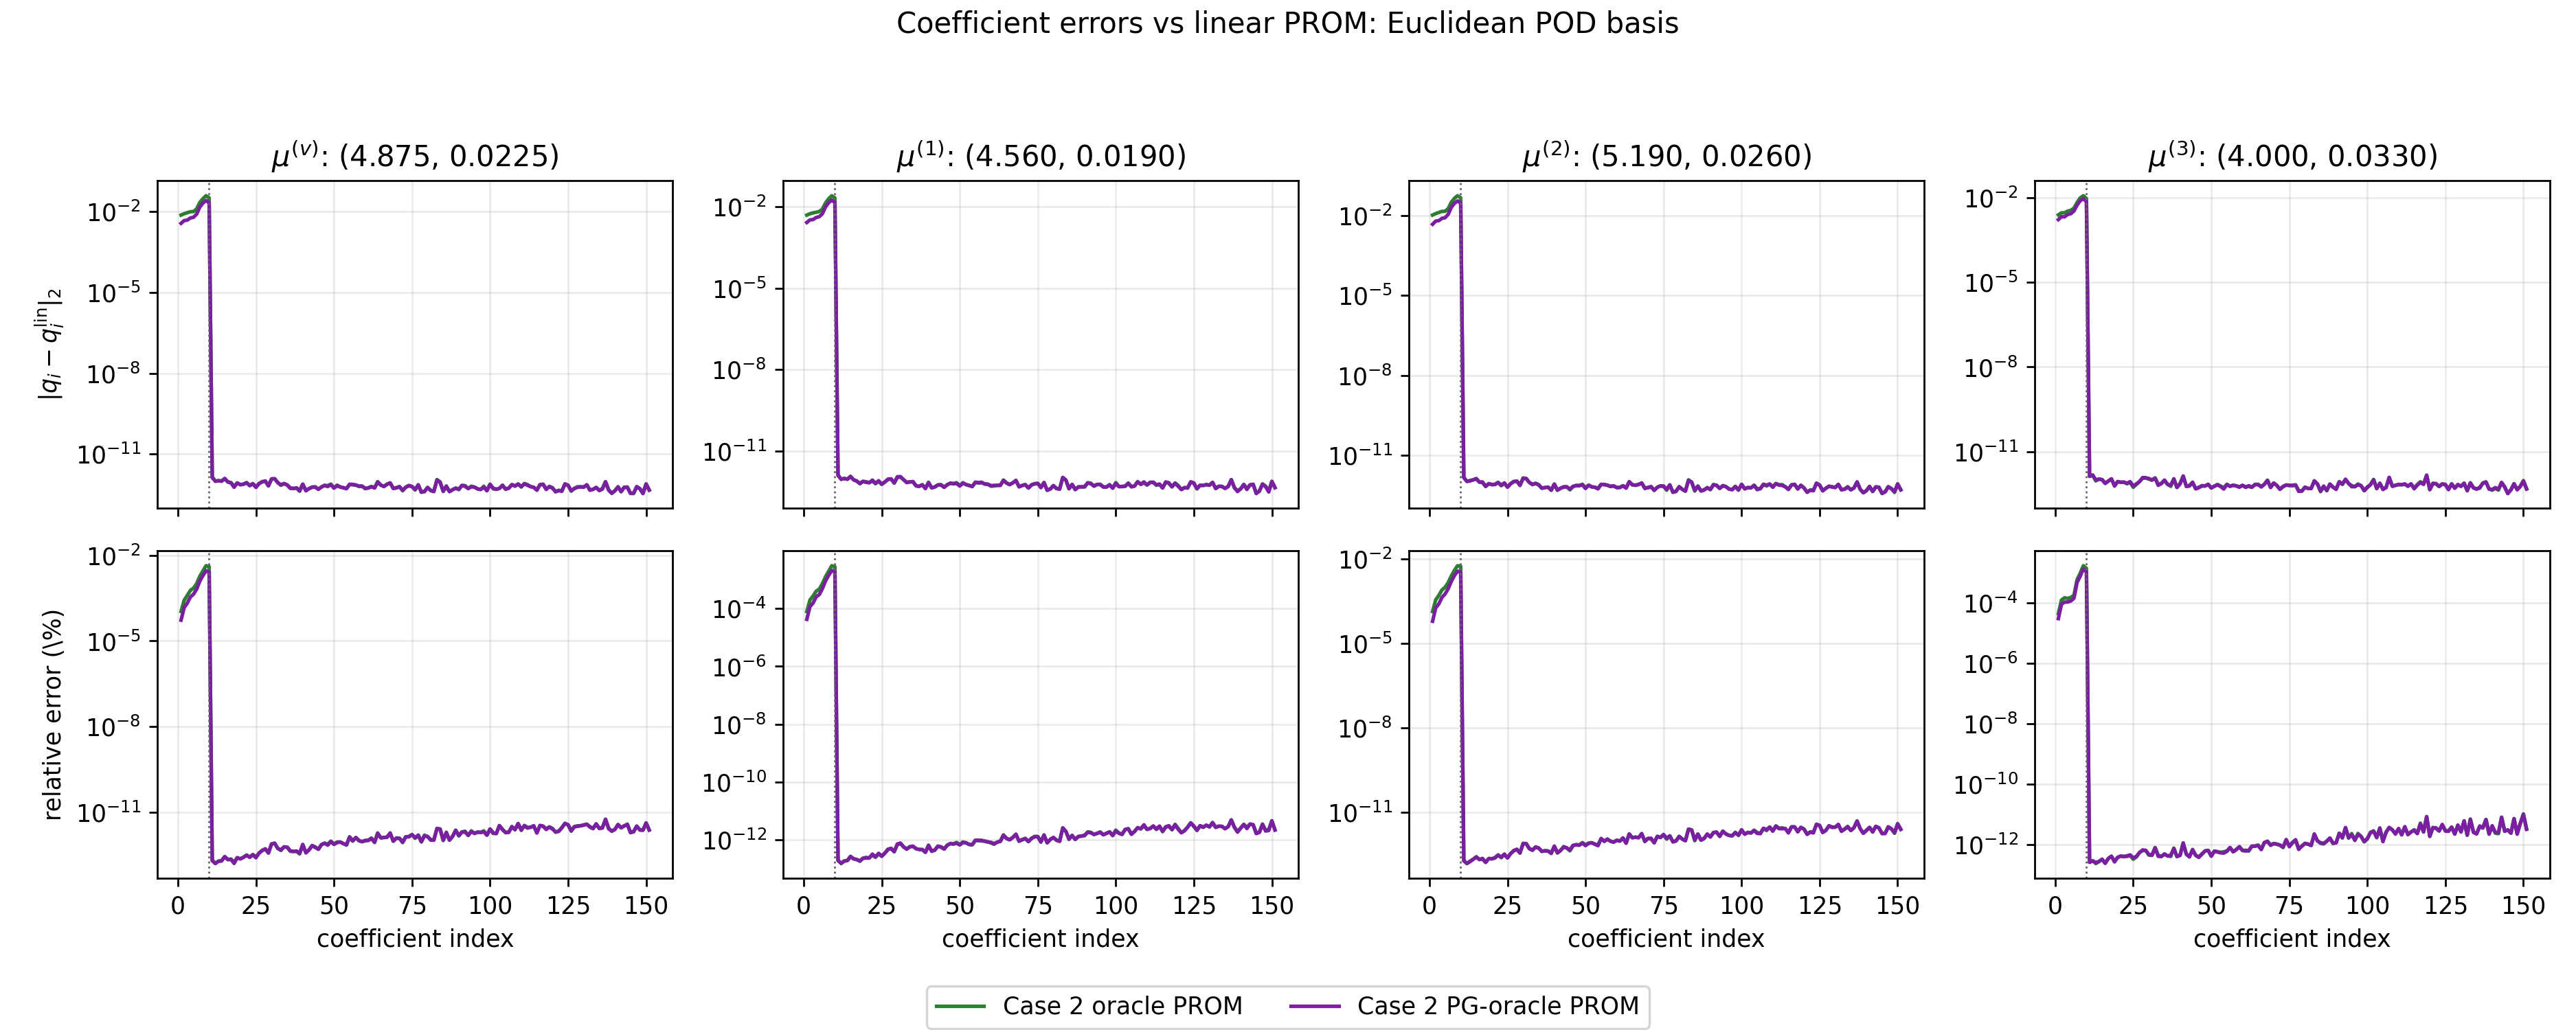
\includegraphics[width=0.98\textwidth]{figures/euclidean_case2_coeff_abs_rel_curves.png}
\caption{Per-coefficient absolute and relative errors with respect to the linear PROM coefficient trajectory.  The dotted line marks the primary/secondary split at $n=10$.}
\end{figure}

\begin{figure}[H]
\centering
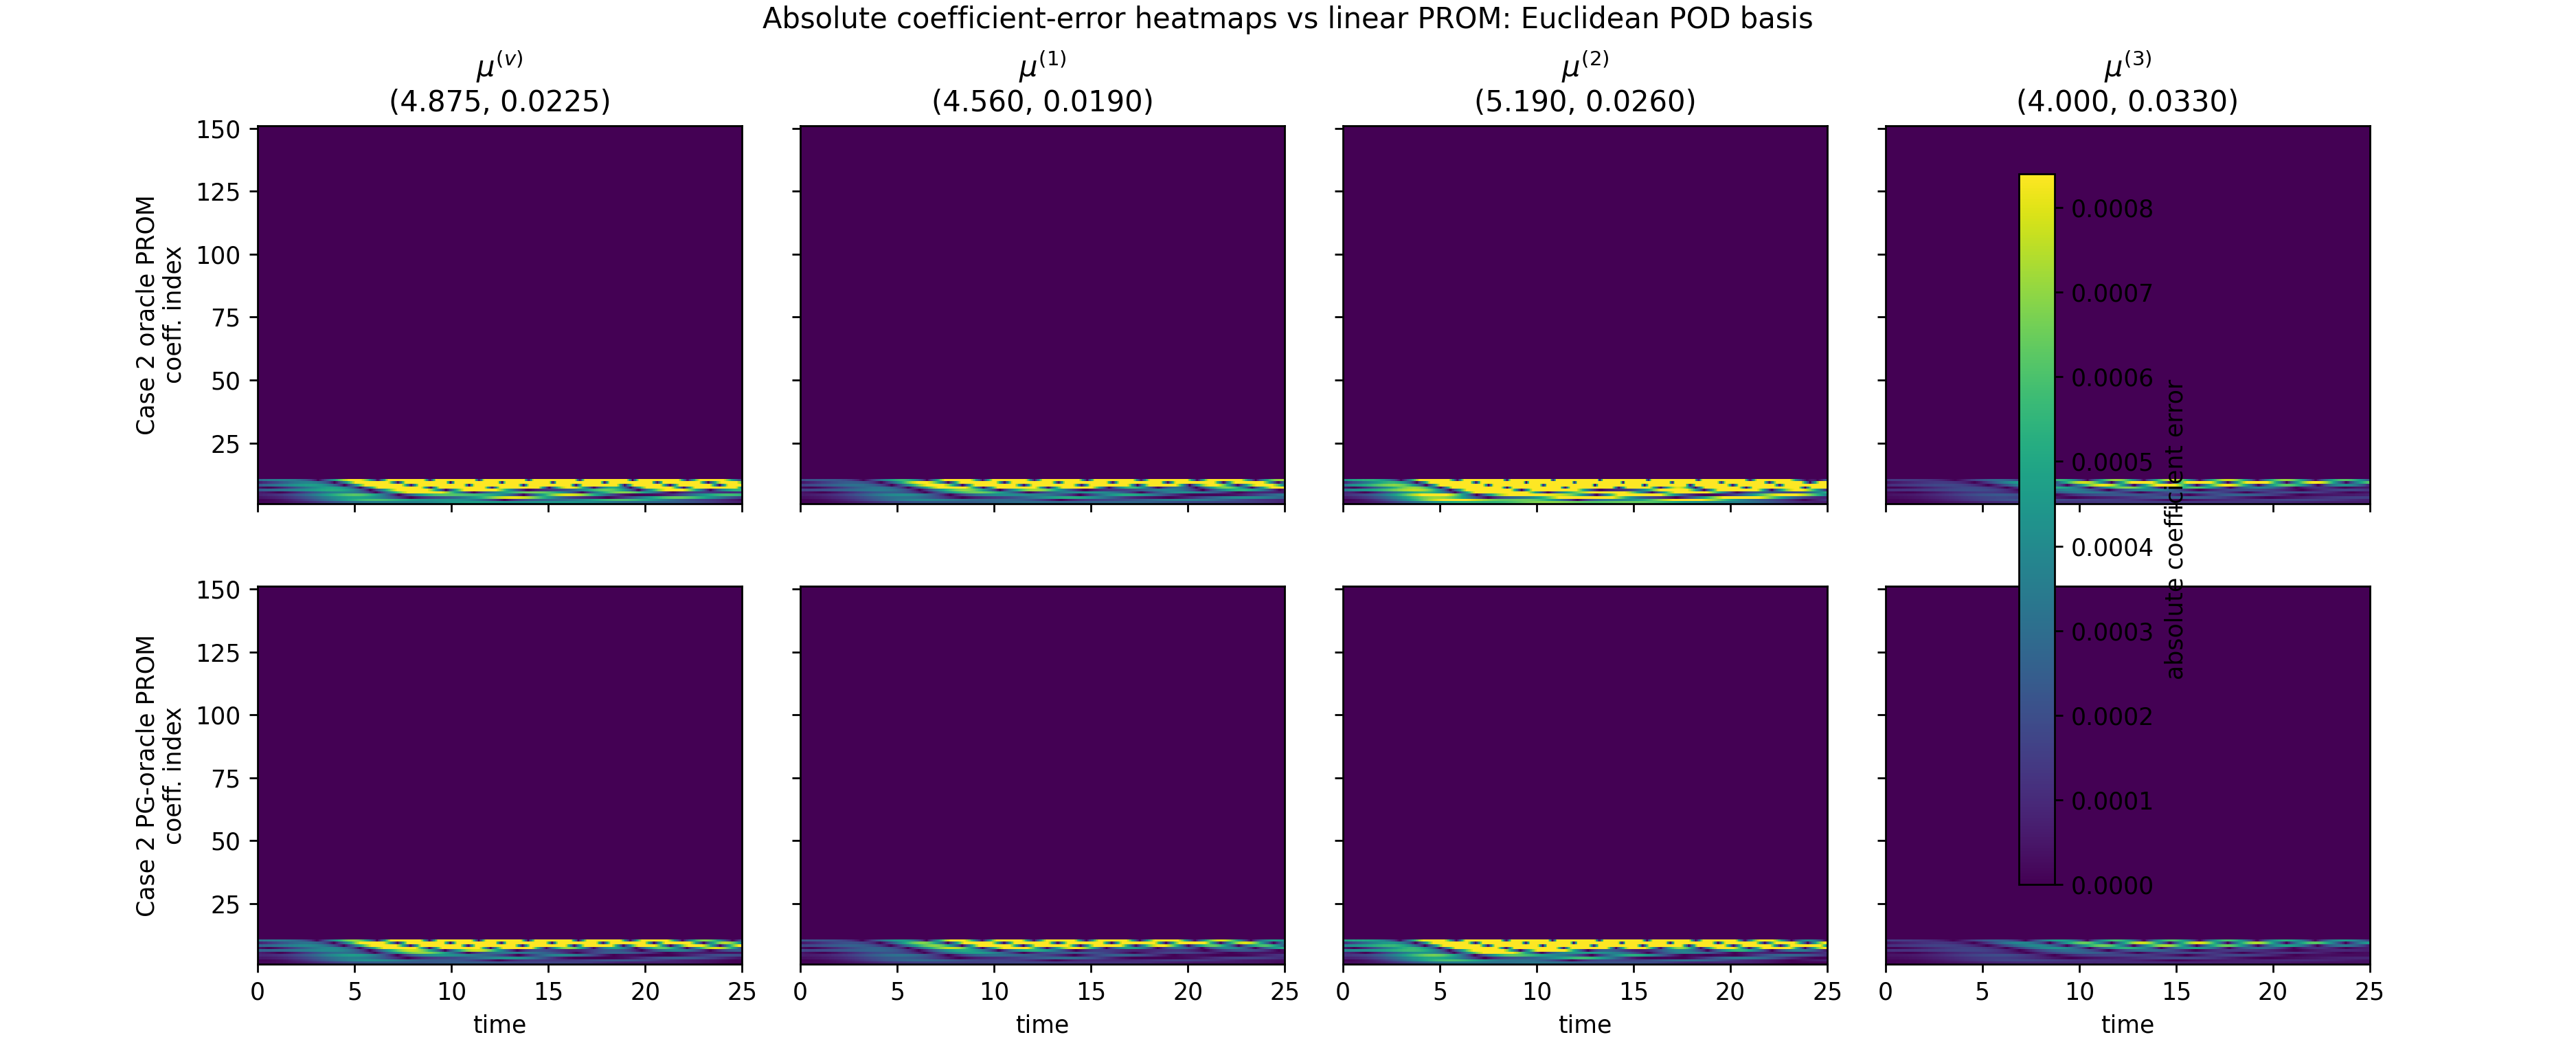
\includegraphics[width=0.98\textwidth]{figures/euclidean_case2_coeff_abs_heatmaps.png}
\caption{Absolute coefficient-error heatmaps versus the linear PROM coefficient trajectory.}
\end{figure}

\begin{figure}[H]
\centering
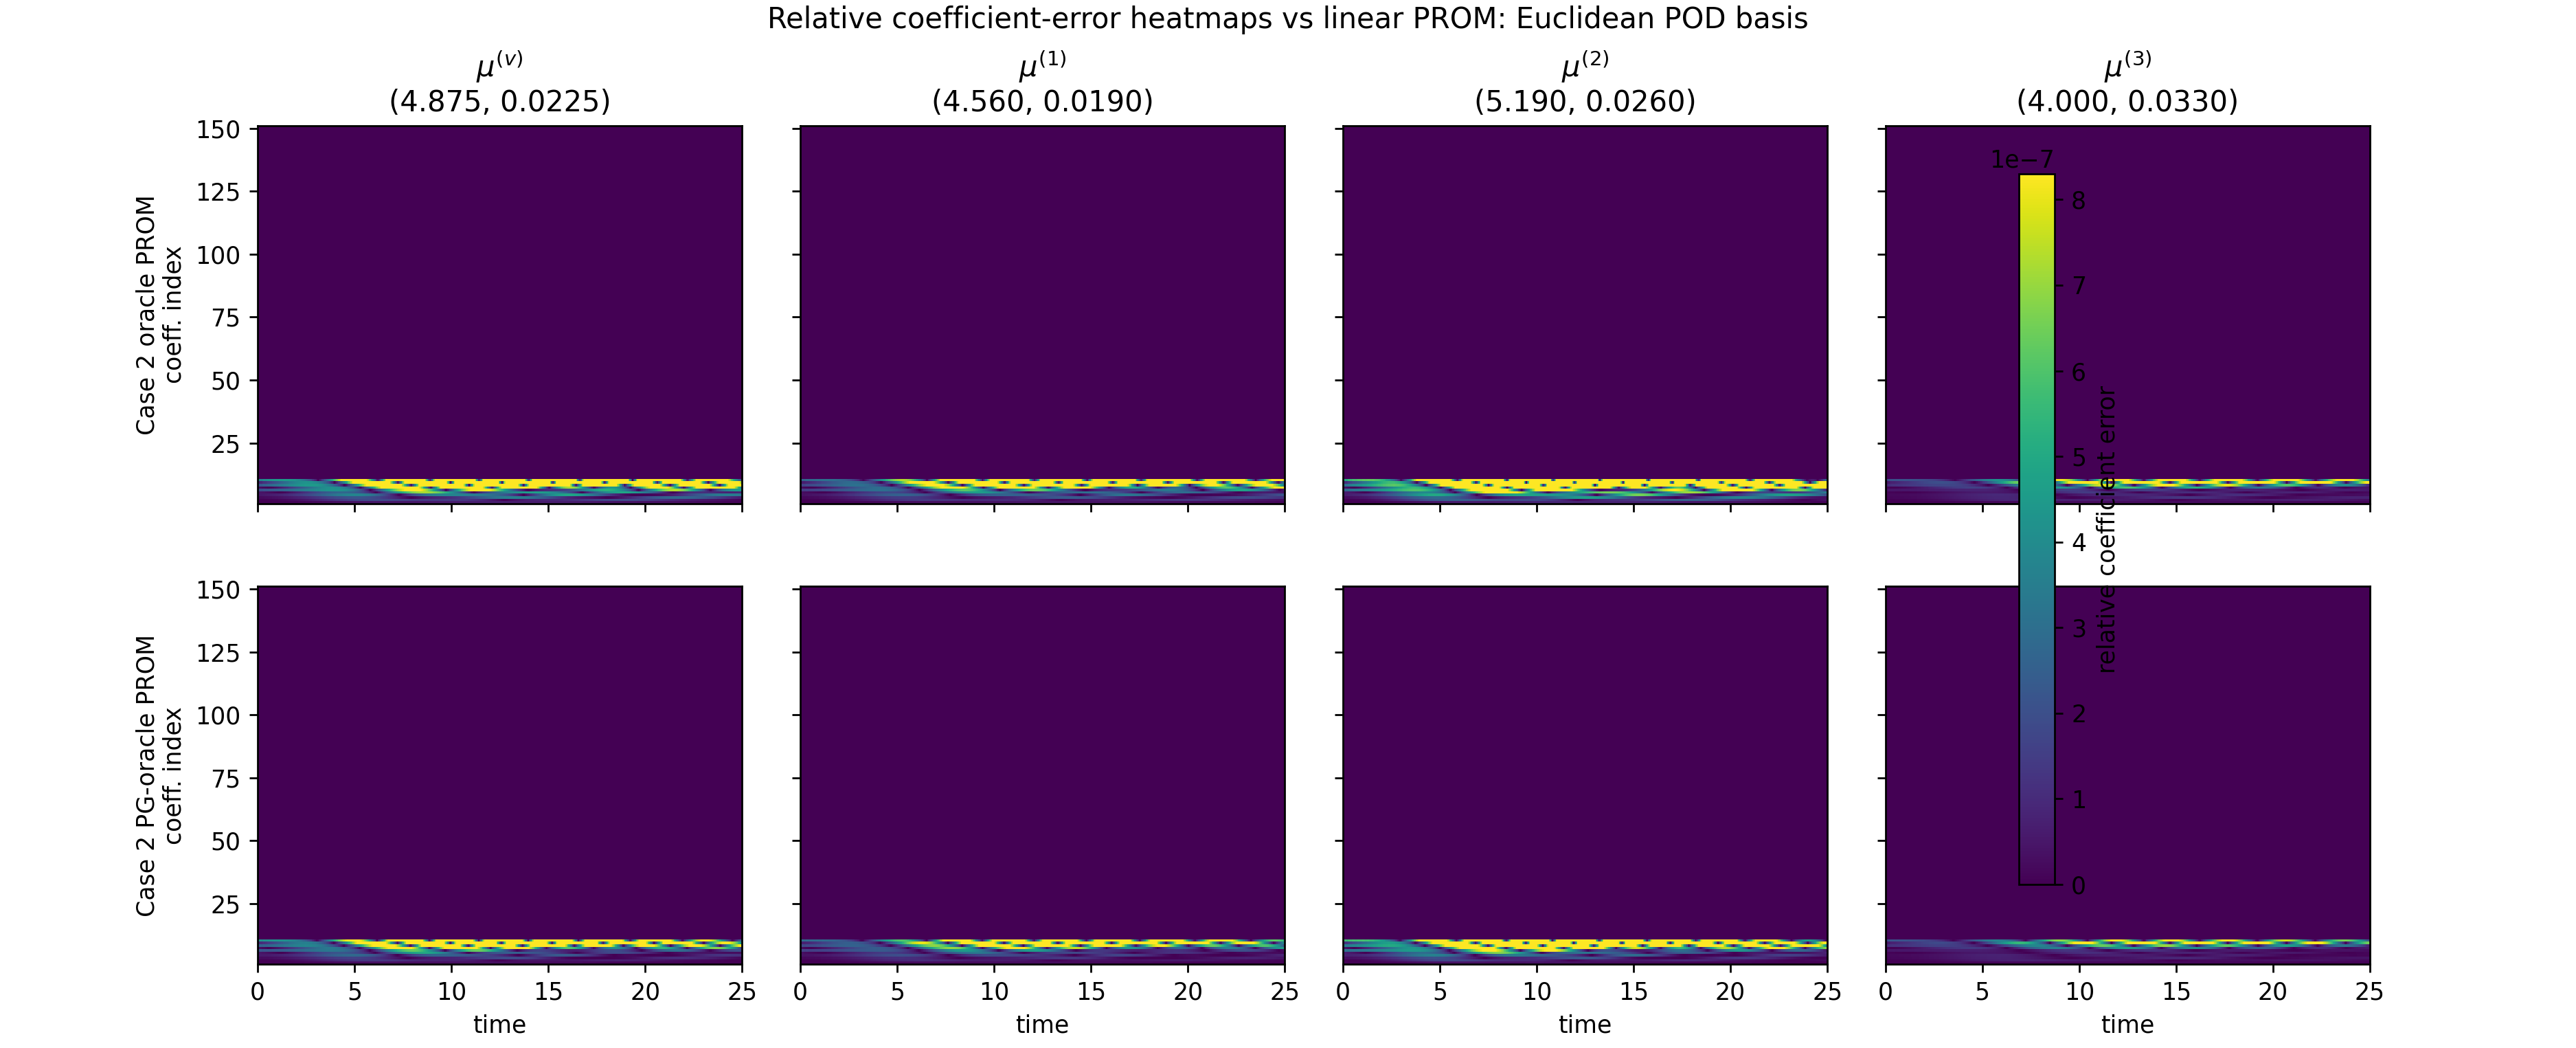
\includegraphics[width=0.98\textwidth]{figures/euclidean_case2_coeff_rel_heatmaps.png}
\caption{Relative coefficient-error heatmaps versus the linear PROM coefficient trajectory.}
\end{figure}

\paragraph{Interpretation.}
For the Euclidean POD basis, the completed corrected test gives the same limiting behavior: both oracle variants nearly coincide with the corresponding linear PROM at all four points.  This is expected because the Euclidean split is essentially orthogonal and the corrected initialization is consistent with the injected secondary block.


\section*{Overall conclusion}
After correcting the Case~2 initialization, the completed MLSPG-sensitive and
Euclidean oracle-only PROM tests both recover their corresponding linear PROM
trajectories to essentially zero error relative to the linear PROM.  The
diagnostic therefore confirms that prescribing the exact secondary coordinates
is sufficient to recover the linear PROM trajectory.  The previously observed
MLSPG oracle discrepancy was caused by an inconsistent initial primary
coordinate, not by a structural failure of the Case~2 reduced problem.
Consequently, Case~2 production errors should be interpreted as neural-network
secondary-coordinate regression error and its online feedback.

\end{document}
